\documentclass{standalone}
\usepackage{tikz}
\usetikzlibrary{patterns, positioning}


\begin{document}
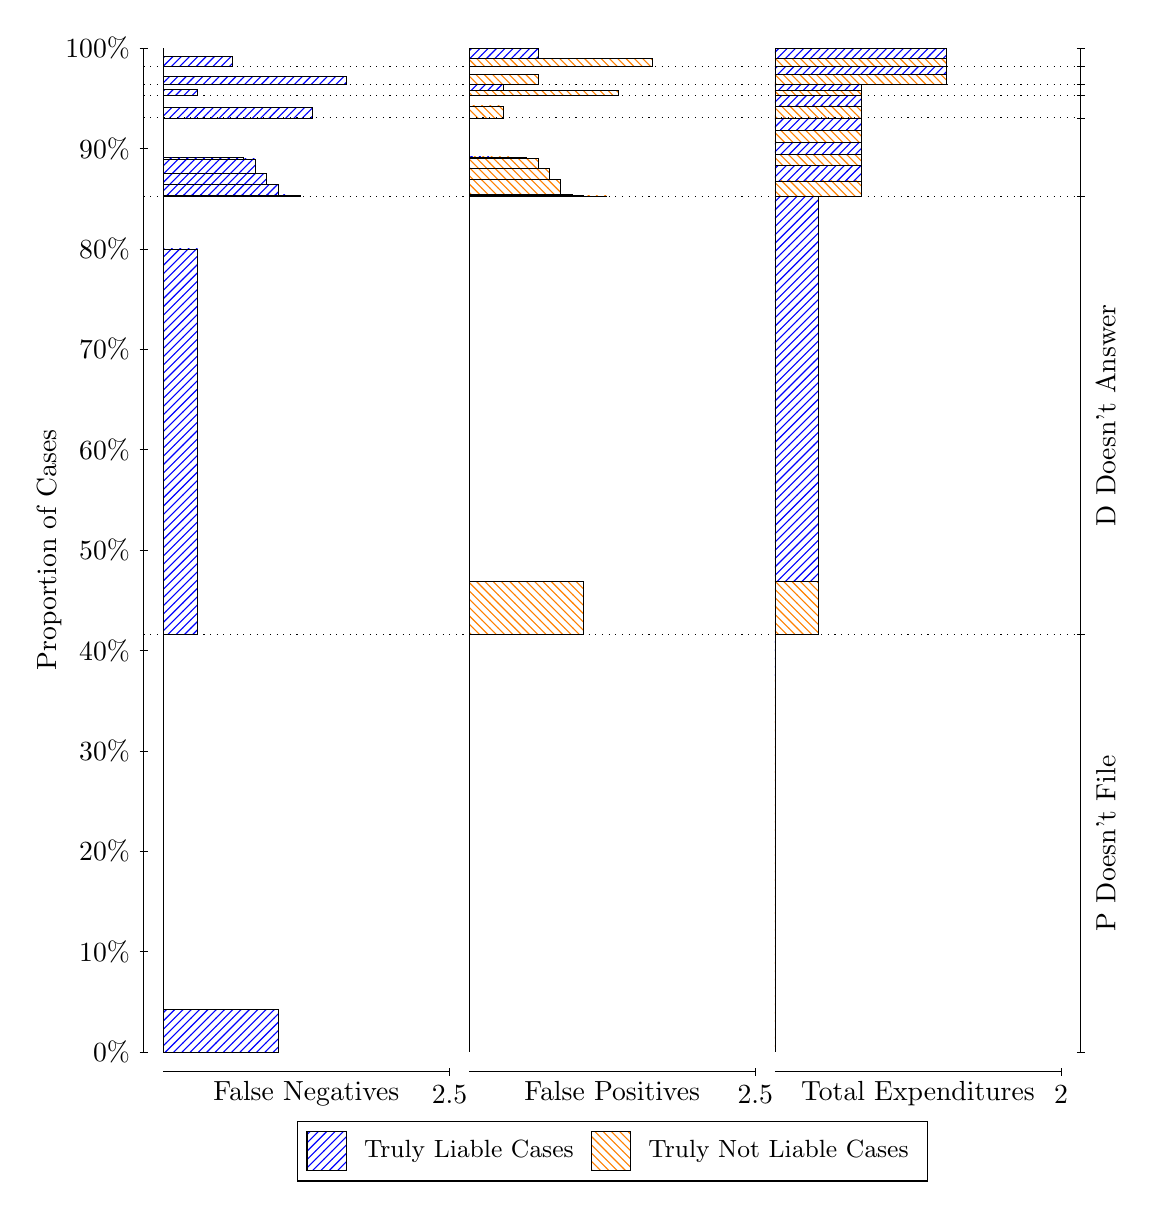
\begin{tikzpicture}
\draw[black, very thin] (1.5,1.75) -- (1.5,14.5);
\node[rotate=90, text=black, anchor=center] at (0.3, 8.125) {Proportion of Cases};
\draw[black, very thin] (1.45,1.75) -- (1.55,1.75);
\node[text=black, anchor=east] at (1.45, 1.75) {0\%};
\draw[black, very thin] (1.45,3.025) -- (1.55,3.025);
\node[text=black, anchor=east] at (1.45, 3.025) {10\%};
\draw[black, very thin] (1.45,4.3) -- (1.55,4.3);
\node[text=black, anchor=east] at (1.45, 4.3) {20\%};
\draw[black, very thin] (1.45,5.575) -- (1.55,5.575);
\node[text=black, anchor=east] at (1.45, 5.575) {30\%};
\draw[black, very thin] (1.45,6.85) -- (1.55,6.85);
\node[text=black, anchor=east] at (1.45, 6.85) {40\%};
\draw[black, very thin] (1.45,8.125) -- (1.55,8.125);
\node[text=black, anchor=east] at (1.45, 8.125) {50\%};
\draw[black, very thin] (1.45,9.4) -- (1.55,9.4);
\node[text=black, anchor=east] at (1.45, 9.4) {60\%};
\draw[black, very thin] (1.45,10.675) -- (1.55,10.675);
\node[text=black, anchor=east] at (1.45, 10.675) {70\%};
\draw[black, very thin] (1.45,11.95) -- (1.55,11.95);
\node[text=black, anchor=east] at (1.45, 11.95) {80\%};
\draw[black, very thin] (1.45,13.225) -- (1.55,13.225);
\node[text=black, anchor=east] at (1.45, 13.225) {90\%};
\draw[black, very thin] (1.45,14.5) -- (1.55,14.5);
\node[text=black, anchor=east] at (1.45, 14.5) {100\%};

\draw[black, very thin] (13.4,1.75) -- (13.4,14.5);
\draw[black, very thin] (13.35,1.75) -- (13.45,1.75);
\node[anchor=west] at (13.35, 1.75) {};
\draw[black, very thin] (13.35,7.0516) -- (13.45,7.0516);
\node[anchor=west] at (13.35, 7.0516) {};
\draw[black, very thin] (13.35,12.62) -- (13.45,12.62);
\node[anchor=west] at (13.35, 12.62) {};
\draw[black, very thin] (13.35,13.613) -- (13.45,13.613);
\node[anchor=west] at (13.35, 13.613) {};
\draw[black, very thin] (13.35,13.901) -- (13.45,13.901);
\node[anchor=west] at (13.35, 13.901) {};
\draw[black, very thin] (13.35,14.036) -- (13.45,14.036);
\node[anchor=west] at (13.35, 14.036) {};
\draw[black, very thin] (13.35,14.266) -- (13.45,14.266);
\node[anchor=west] at (13.35, 14.266) {};
\draw[black, very thin] (13.35,14.5) -- (13.45,14.5);
\node[anchor=west] at (13.35, 14.5) {};

\draw[black, very thin, pattern color=blue, pattern=north east lines] (1.75,1.75) rectangle (3.2033,2.2912);
\draw[black, very thin, pattern color=orange, pattern=north west lines] (1.75,2.2912) rectangle (1.75,7.0516);
\draw[black, very thin, pattern color=blue, pattern=north east lines] (1.75,7.0516) rectangle (2.186,11.948);
\draw[black, very thin, pattern color=orange, pattern=north west lines] (1.75,11.948) rectangle (1.75,12.62);
\draw[black, very thin, pattern color=blue, pattern=north east lines] (1.75,12.62) rectangle (3.494,12.625);
\draw[black, very thin, pattern color=blue, pattern=north east lines] (1.75,12.625) rectangle (3.3487,12.635);
\draw[black, very thin, pattern color=blue, pattern=north east lines] (1.75,12.635) rectangle (3.2033,12.765);
\draw[black, very thin, pattern color=blue, pattern=north east lines] (1.75,12.765) rectangle (3.058,12.766);
\draw[black, very thin, pattern color=blue, pattern=north east lines] (1.75,12.766) rectangle (3.058,12.905);
\draw[black, very thin, pattern color=blue, pattern=north east lines] (1.75,12.905) rectangle (2.9127,13.092);
\draw[black, very thin, pattern color=blue, pattern=north east lines] (1.75,13.092) rectangle (2.7673,13.111);
\draw[black, very thin, pattern color=blue, pattern=north east lines] (1.75,13.111) rectangle (2.622,13.115);
\draw[black, very thin, pattern color=blue, pattern=north east lines] (1.75,13.115) rectangle (2.4767,13.116);
\draw[black, very thin, pattern color=blue, pattern=north east lines] (1.75,13.116) rectangle (2.3313,13.116);
\draw[black, very thin, pattern color=orange, pattern=north west lines] (1.75,13.116) rectangle (1.75,13.613);
\draw[black, very thin, pattern color=blue, pattern=north east lines] (1.75,13.613) rectangle (3.6393,13.75);
\draw[black, very thin, pattern color=orange, pattern=north west lines] (1.75,13.75) rectangle (1.75,13.901);
\draw[black, very thin, pattern color=blue, pattern=north east lines] (1.75,13.901) rectangle (2.186,13.973);
\draw[black, very thin, pattern color=orange, pattern=north west lines] (1.75,13.973) rectangle (1.75,14.036);
\draw[black, very thin, pattern color=blue, pattern=north east lines] (1.75,14.036) rectangle (4.0753,14.141);
\draw[black, very thin, pattern color=orange, pattern=north west lines] (1.75,14.141) rectangle (1.75,14.266);
\draw[black, very thin, pattern color=blue, pattern=north east lines] (1.75,14.266) rectangle (2.622,14.395);
\draw[black, very thin, pattern color=orange, pattern=north west lines] (1.75,14.395) rectangle (1.75,14.5);
\draw[black, very thin, pattern color=orange, pattern=north west lines] (5.6333,1.75) rectangle (5.6333,6.5104);
\draw[black, very thin, pattern color=blue, pattern=north east lines] (5.6333,6.5104) rectangle (5.6333,7.0516);
\draw[black, very thin, pattern color=orange, pattern=north west lines] (5.6333,7.0516) rectangle (7.0867,7.724);
\draw[black, very thin, pattern color=blue, pattern=north east lines] (5.6333,7.724) rectangle (5.6333,12.62);
\draw[black, very thin, pattern color=orange, pattern=north west lines] (5.6333,12.62) rectangle (7.3773,12.621);
\draw[black, very thin, pattern color=orange, pattern=north west lines] (5.6333,12.621) rectangle (7.232,12.621);
\draw[black, very thin, pattern color=orange, pattern=north west lines] (5.6333,12.621) rectangle (7.0867,12.626);
\draw[black, very thin, pattern color=orange, pattern=north west lines] (5.6333,12.626) rectangle (6.9413,12.644);
\draw[black, very thin, pattern color=orange, pattern=north west lines] (5.6333,12.644) rectangle (6.796,12.831);
\draw[black, very thin, pattern color=orange, pattern=north west lines] (5.6333,12.831) rectangle (6.6507,12.972);
\draw[black, very thin, pattern color=orange, pattern=north west lines] (5.6333,12.972) rectangle (6.5053,13.101);
\draw[black, very thin, pattern color=orange, pattern=north west lines] (5.6333,13.101) rectangle (6.36,13.111);
\draw[black, very thin, pattern color=orange, pattern=north west lines] (5.6333,13.111) rectangle (6.2147,13.117);
\draw[black, very thin, pattern color=blue, pattern=north east lines] (5.6333,13.117) rectangle (5.924,13.118);
\draw[black, very thin, pattern color=blue, pattern=north east lines] (5.6333,13.118) rectangle (5.7787,13.118);
\draw[black, very thin, pattern color=blue, pattern=north east lines] (5.6333,13.118) rectangle (5.6333,13.613);
\draw[black, very thin, pattern color=orange, pattern=north west lines] (5.6333,13.613) rectangle (6.0693,13.765);
\draw[black, very thin, pattern color=blue, pattern=north east lines] (5.6333,13.765) rectangle (5.6333,13.901);
\draw[black, very thin, pattern color=orange, pattern=north west lines] (5.6333,13.901) rectangle (7.5227,13.965);
\draw[black, very thin, pattern color=blue, pattern=north east lines] (5.6333,13.965) rectangle (6.0693,14.036);
\draw[black, very thin, pattern color=orange, pattern=north west lines] (5.6333,14.036) rectangle (6.5053,14.162);
\draw[black, very thin, pattern color=blue, pattern=north east lines] (5.6333,14.162) rectangle (5.6333,14.266);
\draw[black, very thin, pattern color=orange, pattern=north west lines] (5.6333,14.266) rectangle (7.9587,14.371);
\draw[black, very thin, pattern color=blue, pattern=north east lines] (5.6333,14.371) rectangle (6.5053,14.5);
\draw[black, very thin, pattern color=orange, pattern=north west lines] (9.5167,1.75) rectangle (9.5167,6.5104);
\draw[black, very thin, pattern color=blue, pattern=north east lines] (9.5167,6.5104) rectangle (9.5167,7.0516);
\draw[black, very thin, pattern color=orange, pattern=north west lines] (9.5167,7.0516) rectangle (10.062,7.724);
\draw[black, very thin, pattern color=blue, pattern=north east lines] (9.5167,7.724) rectangle (10.062,12.62);
\draw[black, very thin, pattern color=orange, pattern=north west lines] (9.5167,12.62) rectangle (10.607,12.813);
\draw[black, very thin, pattern color=blue, pattern=north east lines] (9.5167,12.813) rectangle (10.607,13.005);
\draw[black, very thin, pattern color=orange, pattern=north west lines] (9.5167,13.005) rectangle (10.607,13.151);
\draw[black, very thin, pattern color=blue, pattern=north east lines] (9.5167,13.151) rectangle (10.607,13.297);
\draw[black, very thin, pattern color=orange, pattern=north west lines] (9.5167,13.297) rectangle (10.607,13.455);
\draw[black, very thin, pattern color=blue, pattern=north east lines] (9.5167,13.455) rectangle (10.607,13.613);
\draw[black, very thin, pattern color=orange, pattern=north west lines] (9.5167,13.613) rectangle (10.607,13.765);
\draw[black, very thin, pattern color=blue, pattern=north east lines] (9.5167,13.765) rectangle (10.607,13.901);
\draw[black, very thin, pattern color=orange, pattern=north west lines] (9.5167,13.901) rectangle (10.607,13.965);
\draw[black, very thin, pattern color=blue, pattern=north east lines] (9.5167,13.965) rectangle (10.607,14.036);
\draw[black, very thin, pattern color=orange, pattern=north west lines] (9.5167,14.036) rectangle (11.697,14.162);
\draw[black, very thin, pattern color=blue, pattern=north east lines] (9.5167,14.162) rectangle (11.697,14.266);
\draw[black, very thin, pattern color=orange, pattern=north west lines] (9.5167,14.266) rectangle (11.697,14.371);
\draw[black, very thin, pattern color=blue, pattern=north east lines] (9.5167,14.371) rectangle (11.697,14.5);
\draw[black, dotted] (1.5,7.0516) -- (13.4,7.0516);
\draw[black, dotted] (1.5,12.62) -- (13.4,12.62);
\draw[black, dotted] (1.5,13.613) -- (13.4,13.613);
\draw[black, dotted] (1.5,13.901) -- (13.4,13.901);
\draw[black, dotted] (1.5,14.036) -- (13.4,14.036);
\draw[black, dotted] (1.5,14.266) -- (13.4,14.266);
\draw[black, very thin] (1.75,1.5) -- (5.3833,1.5);
\node[text=black, anchor=north] at (3.5667, 1.5) {False Negatives};
\draw[black, very thin] (5.3833,1.45) -- (5.3833,1.55);
\node[text=black, anchor=north] at (5.3833, 1.45) {2.5};

\draw[black, very thin] (5.6333,1.5) -- (9.2667,1.5);
\node[text=black, anchor=north] at (7.45, 1.5) {False Positives};
\draw[black, very thin] (9.2667,1.45) -- (9.2667,1.55);
\node[text=black, anchor=north] at (9.2667, 1.45) {2.5};

\draw[black, very thin] (9.5167,1.5) -- (13.15,1.5);
\node[text=black, anchor=north] at (11.333, 1.5) {Total Expenditures};
\draw[black, very thin] (13.15,1.45) -- (13.15,1.55);
\node[text=black, anchor=north] at (13.15, 1.45) {2};

\node[text=black, centered, rotate=90] at (13.72, 4.4008) {P Doesn't File};
\node[text=black, centered, rotate=90] at (13.72, 9.836) {D Doesn't Answer};






\draw (7.449999999999999,1.5) node[draw=none] (baseCoordinate) {};
\begin{scope}[align=center]
        \matrix[scale=0.5, draw=black, below=0.5cm of baseCoordinate, nodes={draw}, column sep=0.1cm]{
            \node[rectangle, draw, minimum width=0.5cm, minimum height=0.5cm, pattern color=blue, pattern=north east lines] {}; &
            \node[draw=none, font=\small, text=black] (B) {Truly Liable Cases}; &
            \node[rectangle, draw, minimum width=0.5cm, minimum height=0.5cm, pattern color=orange, pattern=north west lines] {}; &
            \node[draw=none, font=\small, text=black] (B) {Truly Not Liable Cases}; \\
            };
\end{scope}

\end{tikzpicture}
\end{document}